\documentclass[border=8pt,tikz]{standalone}
\usepackage{fontspec}
\usepackage{babel}
\babelprovide[import, main]{vietnamese}
\babelfont{rm}{Latin Modern Roman}
\babelfont{sf}{Latin Modern Roman}
\babelfont{tt}{Latin Modern Roman}
\usepackage{tikz}
\usetikzlibrary{arrows.meta,calc,positioning,backgrounds}

\definecolor{navy}{HTML}{0F2C59}
\definecolor{deepblue}{HTML}{1D4ED8}
\definecolor{teal}{HTML}{0D9488}
\definecolor{darkteal}{HTML}{0F766E}
\definecolor{crimson}{HTML}{DC2626}
\definecolor{amber}{HTML}{D97706}
\definecolor{gold}{HTML}{F59E0B}
\definecolor{purple}{HTML}{6D28D9}
\definecolor{slate}{HTML}{334155}
\definecolor{lightgray}{HTML}{F8FAFC}
\definecolor{softblue}{HTML}{EEF4FE}
\definecolor{softteal}{HTML}{EBF9F6}
\definecolor{softred}{HTML}{FEF0F0}
\definecolor{softamber}{HTML}{FEF7E6}
\definecolor{softpurple}{HTML}{F4EFFE}

\begin{document}
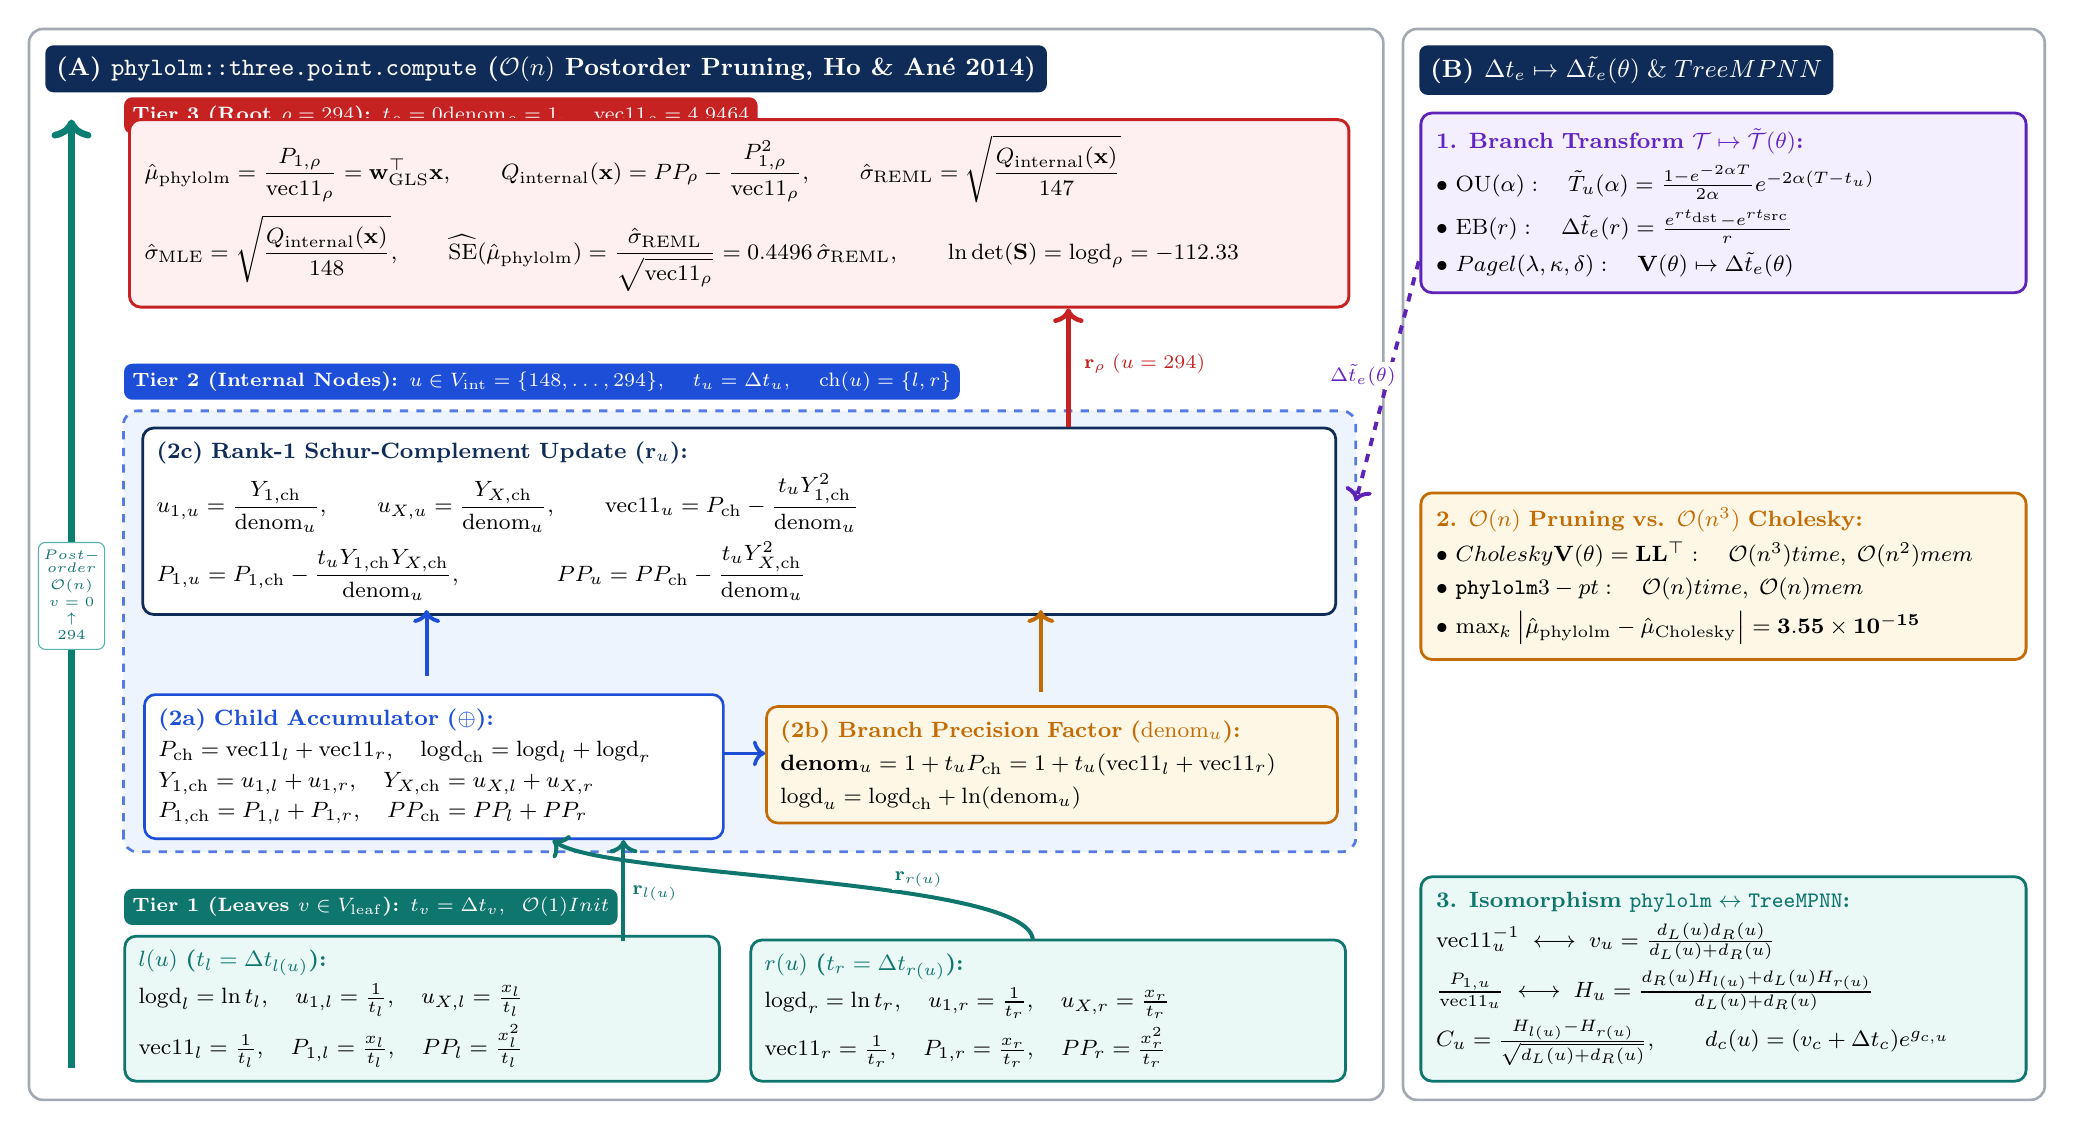
\begin{tikzpicture}

% ==============================================================================
% PANEL (A): 3-TIER BOTTOM-UP POSTORDER PRUNING FLOWCHART (PURE FORMULAS)
% ==============================================================================
\filldraw[fill=white, draw=slate!45, line width=0.95pt, rounded corners=5pt] (0.00,0.00) rectangle (17.20,13.60);
\node[fill=navy, text=white, rounded corners=3pt, inner sep=4pt, anchor=north west, font=\small\bfseries]
    at (0.20,13.40) {(A) \texttt{phylolm::three.point.compute} ($\mathcal{O}(n)$ Postorder Pruning, Ho \& Ané 2014)};

% Left Vertical Postorder Traversal Arrow (Bottom -> Top)
\draw[->, draw=teal!85!black, line width=2.4pt] (0.54,0.40) -- (0.54,12.45);
\node[fill=white, draw=teal!70, rounded corners=2.5pt, inner sep=1.8pt, text=darkteal, anchor=center, font=\tiny\bfseries]
    at (0.54,6.40) {$\begin{array}{@{}c@{}}\text{Post-}\\[-1pt]\text{order}\\\mathcal{O}(n)\\v=0\\\uparrow\\294\end{array}$};

% ------------------------------------------------------------------------------
% TIER 1 (BOTTOM): O(1) LEAF REGISTERS (v in V_leaf = {0..147})
% ------------------------------------------------------------------------------
\node[fill=darkteal, text=white, rounded corners=3pt, inner sep=3pt, anchor=west, font=\scriptsize\bfseries]
    at (1.20,2.45) {Tier 1 (Leaves $v \in V_{\mathrm{leaf}}$): $t_v = \Delta t_v,\;\; \mathcal{O}(1)\text{ Init}$};

\node[fill=softteal, draw=darkteal, line width=1.0pt, rounded corners=4pt, inner sep=5pt, text width=7.2cm, anchor=south west, font=\footnotesize]
    at (1.20,0.22) {
    {\bfseries\color{darkteal} $l(u)$ ($t_l = \Delta t_{l(u)}$):}\\[2pt]
    $\mathrm{logd}_l = \ln t_l,\quad u_{1,l} = \frac{1}{t_l},\quad u_{X,l} = \frac{x_l}{t_l}$\\[2pt]
    $\mathrm{vec11}_l = \frac{1}{t_l},\quad P_{1,l} = \frac{x_l}{t_l},\quad PP_l = \frac{x_l^2}{t_l}$
};

\node[fill=softteal, draw=darkteal, line width=1.0pt, rounded corners=4pt, inner sep=5pt, text width=7.2cm, anchor=south west, font=\footnotesize]
    at (9.15,0.22) {
    {\bfseries\color{darkteal} $r(u)$ ($t_r = \Delta t_{r(u)}$):}\\[2pt]
    $\mathrm{logd}_r = \ln t_r,\quad u_{1,r} = \frac{1}{t_r},\quad u_{X,r} = \frac{x_r}{t_r}$\\[2pt]
    $\mathrm{vec11}_r = \frac{1}{t_r},\quad P_{1,r} = \frac{x_r}{t_r},\quad PP_r = \frac{x_r^2}{t_r}$
};

% ------------------------------------------------------------------------------
% TIER 2 (MIDDLE): RECURSIVE MERGE AT 147 INTERNAL NODES (u = 148 -> 294)
% ------------------------------------------------------------------------------
\node[fill=deepblue, text=white, rounded corners=3pt, inner sep=3pt, anchor=west, font=\scriptsize\bfseries]
    at (1.20,9.12) {Tier 2 (Internal Nodes): $u \in V_{\mathrm{int}} = \{148,\dots,294\},\quad t_u = \Delta t_u,\quad \mathrm{ch}(u)=\{l,r\}$};

\filldraw[fill=softblue, draw=deepblue!75, line width=1.0pt, rounded corners=5pt, dashed]
    (1.20,3.15) rectangle (16.85,8.75);

% Step 2a (Left) and Step 2b (Right)
\node[fill=white, draw=deepblue, line width=0.95pt, rounded corners=4pt, inner sep=5pt, text width=7.0cm, anchor=south west, font=\footnotesize]
    at (1.45,3.30) {
    {\bfseries\color{deepblue} (2a) Child Accumulator ($\oplus$):}\\[2pt]
    $P_{\mathrm{ch}} = \mathrm{vec11}_l + \mathrm{vec11}_r,\quad \mathrm{logd}_{\mathrm{ch}} = \mathrm{logd}_l + \mathrm{logd}_r$\\[1.5pt]
    $Y_{1,\mathrm{ch}} = u_{1,l} + u_{1,r},\quad Y_{X,\mathrm{ch}} = u_{X,l} + u_{X,r}$\\[1.5pt]
    $P_{1,\mathrm{ch}} = P_{1,l} + P_{1,r},\quad PP_{\mathrm{ch}} = PP_l + PP_r$
};

\node[fill=softamber, draw=amber!90!black, line width=0.95pt, rounded corners=4pt, inner sep=5pt, text width=6.9cm, anchor=south west, font=\footnotesize]
    at (9.35,3.50) {
    {\bfseries\color{amber!90!black} (2b) Branch Precision Factor ($\mathrm{denom}_u$):}\\[2.5pt]
    $\mathbf{denom}_u = 1 + t_u P_{\mathrm{ch}} = 1 + t_u(\mathrm{vec11}_l + \mathrm{vec11}_r)$\\[2.5pt]
    $\mathrm{logd}_u = \mathrm{logd}_{\mathrm{ch}} + \ln(\mathrm{denom}_u)$
};

% Step 2c (Upper part of Tier 2: Schur-Complement Update)
\node[fill=white, draw=navy, line width=1.0pt, rounded corners=4pt, inner sep=5pt, text width=14.8cm, anchor=north, font=\footnotesize]
    at (9.02,8.55) {
    {\bfseries\color{navy} (2c) Rank-1 Schur-Complement Update ($\mathbf{r}_u$):}\\[2.5pt]
    $\displaystyle
    u_{1,u} = \frac{Y_{1,\mathrm{ch}}}{\mathrm{denom}_u},\qquad
    u_{X,u} = \frac{Y_{X,\mathrm{ch}}}{\mathrm{denom}_u},\qquad
    \mathrm{vec11}_u = P_{\mathrm{ch}} - \frac{t_u Y_{1,\mathrm{ch}}^2}{\mathrm{denom}_u}$\\[2.5pt]
    $\displaystyle
    P_{1,u} = P_{1,\mathrm{ch}} - \frac{t_u Y_{1,\mathrm{ch}}Y_{X,\mathrm{ch}}}{\mathrm{denom}_u},\qquad\qquad
    PP_u = PP_{\mathrm{ch}} - \frac{t_u Y_{X,\mathrm{ch}}^2}{\mathrm{denom}_u}$
};

% Arrows Tier 1 -> Tier 2
\draw[->, draw=darkteal, line width=1.45pt] (7.55,2.02) -- (7.55,3.30);
\node[fill=white, inner sep=1pt, text=darkteal, anchor=west, font=\scriptsize\bfseries] at (7.62,2.62) {$\mathbf{r}_{l(u)}$};

\draw[->, draw=darkteal, line width=1.45pt] (12.75,2.02) .. controls (12.75,2.82) and (7.30,2.82) .. (6.65,3.30);
\node[fill=white, inner sep=1pt, text=darkteal, anchor=west, font=\scriptsize\bfseries] at (10.95,2.80) {$\mathbf{r}_{r(u)}$};

\draw[->, draw=deepblue, line width=1.3pt] (8.80,4.40) -- (9.35,4.40);
\draw[->, draw=deepblue, line width=1.4pt] (5.05,5.38) -- (5.05,6.22);
\draw[->, draw=amber!90!black, line width=1.4pt] (12.85,5.18) -- (12.85,6.22);

% ------------------------------------------------------------------------------
% TIER 3 (TOP): EXACT CLOSED-FORM READOUT AT ROOT rho = 294 (t_rho = 0)
% ------------------------------------------------------------------------------
\node[fill=crimson!90!black, text=white, rounded corners=3pt, inner sep=3pt, anchor=west, font=\scriptsize\bfseries]
    at (1.20,12.50) {Tier 3 (Root $\rho = 294$): $t_\rho = 0 \implies \mathrm{denom}_\rho = 1,\quad \mathrm{vec11}_\rho = 4.9464$};

\node[fill=softred, draw=crimson!90!black, line width=1.05pt, rounded corners=4pt, inner sep=5.5pt, text width=15.1cm, anchor=south, font=\footnotesize]
    at (9.02,10.05) {
    $\displaystyle
    \hat{\mu}_{\mathrm{phylolm}} = \frac{P_{1,\rho}}{\mathrm{vec11}_\rho} = \mathbf{w}_{\mathrm{GLS}}^\top\mathbf{x},\qquad
    Q_{\mathrm{internal}}(\mathbf{x}) = PP_\rho - \frac{P_{1,\rho}^2}{\mathrm{vec11}_\rho},\qquad
    \hat{\sigma}_{\mathrm{REML}} = \sqrt{\frac{Q_{\mathrm{internal}}(\mathbf{x})}{147}}$\\[3.5pt]
    $\displaystyle
    \hat{\sigma}_{\mathrm{MLE}} = \sqrt{\frac{Q_{\mathrm{internal}}(\mathbf{x})}{148}},\qquad
    \widehat{\mathrm{SE}}(\hat{\mu}_{\mathrm{phylolm}}) = \frac{\hat{\sigma}_{\mathrm{REML}}}{\sqrt{\mathrm{vec11}_\rho}} = 0.4496\,\hat{\sigma}_{\mathrm{REML}},\qquad
    \ln\det(\mathbf{S}) = \mathrm{logd}_\rho = -112.33$
};

\draw[->, draw=crimson!90!black, line width=1.65pt] (13.20,8.55) -- (13.20,10.05);
\node[fill=white, inner sep=1.2pt, text=crimson!90!black, anchor=west, font=\scriptsize\bfseries]
    at (13.35,9.35) {$\mathbf{r}_\rho\; (u = 294)$};

% ==============================================================================
% PANEL (B): 3-POINT BRANCH TRANSFORM & GNN ISOMORPHISM (PURE SYMBOLS)
% ==============================================================================
\filldraw[fill=white, draw=slate!45, line width=0.95pt, rounded corners=5pt] (17.45,0.00) rectangle (25.60,13.60);
\node[fill=navy, text=white, rounded corners=3pt, inner sep=4pt, anchor=north west, font=\small\bfseries]
    at (17.65,13.40) {(B) $\Delta t_e \mapsto \Delta\tilde{t}_e(\boldsymbol{\theta})\; \&\; \text{TreeMPNN}$};

% Card 1: 3-Point Branch Length Transform
\node[fill=softpurple, draw=purple!85!black, line width=1.0pt, rounded corners=4pt, inner sep=5.5pt, text width=7.3cm, anchor=north, font=\footnotesize]
    at (21.52,12.55) {
    {\bfseries\color{purple!90!black} 1. Branch Transform $\mathcal{T} \mapsto \tilde{\mathcal{T}}(\boldsymbol{\theta})$:}\\[3pt]
    $\bullet$ $\mathrm{OU}(\alpha):\quad \tilde{T}_u(\alpha) = \frac{1 - e^{-2\alpha T}}{2\alpha}e^{-2\alpha(T - t_u)}$\\[2.5pt]
    $\bullet$ $\mathrm{EB}(r):\quad \Delta\tilde{t}_e(r) = \frac{e^{r t_{\mathrm{dst}}} - e^{r t_{\mathrm{src}}}}{r}$\\[2.5pt]
    $\bullet$ $\text{Pagel }(\lambda,\kappa,\delta):\quad \mathbf{V}(\boldsymbol{\theta}) \mapsto \Delta\tilde{t}_e(\boldsymbol{\theta})$
};

\draw[->, draw=purple!85!black, line width=1.4pt, dashed] (17.65,10.65) -- (16.85,7.60);
\node[fill=white, inner sep=1pt, text=purple!90!black, anchor=east, font=\scriptsize\bfseries] at (17.40,9.20) {$\Delta\tilde{t}_e(\boldsymbol{\theta})$};

% Card 2: Complexity & Precision Comparison
\node[fill=softamber, draw=amber!90!black, line width=1.0pt, rounded corners=4pt, inner sep=5.5pt, text width=7.3cm, anchor=center, font=\footnotesize]
    at (21.52,6.65) {
    {\bfseries\color{amber!90!black} 2. $\mathcal{O}(n)$ Pruning vs. $\mathcal{O}(n^3)$ Cholesky:}\\[3pt]
    $\bullet$ $\text{Cholesky }\mathbf{V}(\boldsymbol{\theta}) = \mathbf{L}\mathbf{L}^\top:\quad \mathcal{O}(n^3)\text{ time},\; \mathcal{O}(n^2)\text{ mem}$\\[2.5pt]
    $\bullet$ $\text{\texttt{phylolm} 3-pt}:\quad \mathcal{O}(n)\text{ time},\; \mathcal{O}(n)\text{ mem}$\\[2.5pt]
    $\bullet$ $\max_{k}\big|\hat{\mu}_{\mathrm{phylolm}} - \hat{\mu}_{\mathrm{Cholesky}}\big| = \mathbf{3.55 \times 10^{-15}}$
};

% Card 3: 1-to-1 Structural Isomorphism to PhyloGNN
\node[fill=softteal, draw=darkteal, line width=1.0pt, rounded corners=4pt, inner sep=5.5pt, text width=7.3cm, anchor=south, font=\footnotesize]
    at (21.52,0.22) {
    {\bfseries\color{darkteal} 3. Isomorphism $\texttt{phylolm} \leftrightarrow \texttt{TreeMPNN}$:}\\[3pt]
    $\mathrm{vec11}_u^{-1} \;\longleftrightarrow\; v_u = \frac{d_L(u)d_R(u)}{d_L(u)+d_R(u)}$\\[2.5pt]
    $\frac{P_{1,u}}{\mathrm{vec11}_u} \;\longleftrightarrow\; H_u = \frac{d_R(u)H_{l(u)} + d_L(u)H_{r(u)}}{d_L(u)+d_R(u)}$\\[2.5pt]
    $C_u = \frac{H_{l(u)} - H_{r(u)}}{\sqrt{d_L(u)+d_R(u)}},\qquad d_{c}(u) = (v_c + \Delta t_c)e^{g_{c,u}}$
};

\end{tikzpicture}
\end{document}
